\chapter{Implementation}\label{ch:method}

\section{Lattice Generation}
While typically one could simply generate a lattice or network at random without any weighting, it is far more interesting to be able to have different starting conditions whereby agents are more likely to be extreme, centralist or any other distribution one wants to test. As such, one can specify their own lattice for analysis or use the beta distribution with varying $\alpha$ and $\beta$ parameters to produce different initial lattices. Interesting beta distributions to try include the uniform distribution ($\alpha = 1$, $\beta = 1$), a more polarised distribution (that is a distribution with higher probability density at the extremes close to 0 and 1) ($\alpha = 0.5$, $\beta = 0.5$) and a more centralist distribution ($\alpha = 2$, $\beta = 2$).

\begin{figure}[H]
\centering
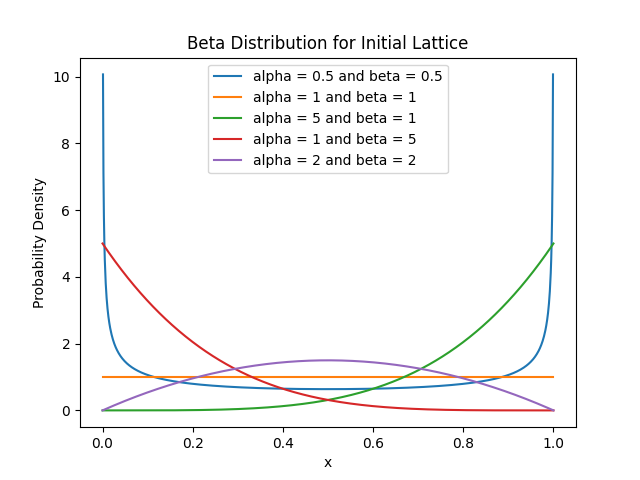
\includegraphics[width = 0.6\textwidth]{Images/Beta Distribution.png}
\caption{The probability density function for various values of $\alpha$ and $\beta$ used in generating the initial lattice. This shows how the initial lattice skews, whether its central or polarised.}
\end{figure}

The code utilises the numpy.random.beta function to produce a lattice of given dimensions (default 50 by 50 if no lattice is specified). An example inital voter lattice is shown below.

\begin{figure}[H]
\centering
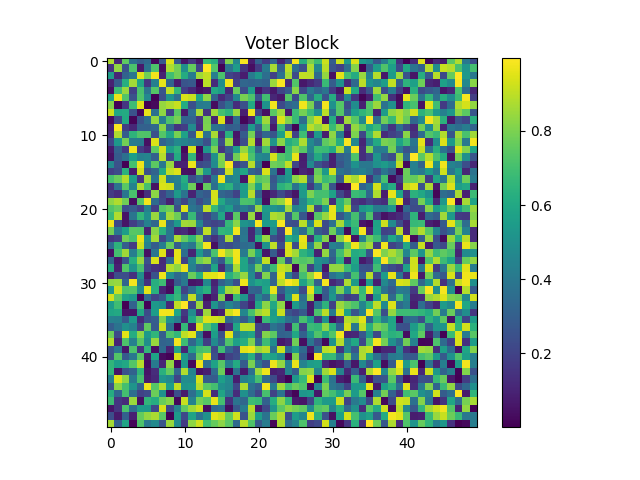
\includegraphics[width=0.6\textwidth]{Images/Example Initial Voter Block.png}
\caption{Example of a Voter Block with $\alpha = 1$ and $\beta = 1$}
\label{beta_dist}
\end{figure}

The lattice generates values from 0 to 1 for each site based on the beta distribution specified. Figure (\ref{beta_dist}) uses $\alpha = 1$ and $\beta = 1$, so every value is equally likely due to the beta distribution being a uniform distribution for these values. An example of a lattice generated with different $\alpha$ and $\beta$ is shown below.

\begin{figure}[H]
\centering
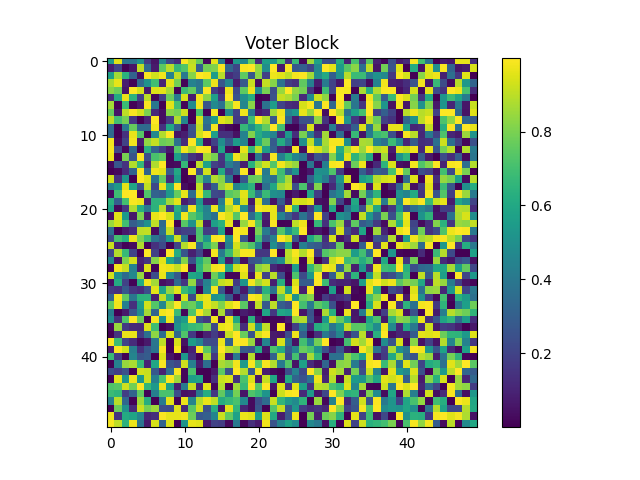
\includegraphics[width=0.6\textwidth]{Images/Example Initial Voter Block 2.png}
\caption{Example of a Voter Block with $\alpha = 0.5$ and $\beta = 0.5$}
\end{figure}

Note how values closer to 0 and 1 are more common for a lattice where the beta distribution used to generate it has $\alpha = 0.5$ and $\beta = 0.5$ than for the lattice where $\alpha = 1$ and $\beta = 1$.

\section{Deffuant Model}
Two different Deffuant models were developed for the code used in this report. One model (which will be referred to as the Deffuant model or normal Deffuant model) simply picks two agents at random (they do not need to be neighbours) and applies the rules/equations \ref{UpRuleA},\ref{UpRuleB} and \ref{CommRequirement}. 

The second developed model is different in how it chooses the two agents. An agent is chosen at random, but one of its four neighbours are chosen at random (without bias) instead of a completely unrelated agent. Then the above rules are applied for updating the lattice. This will be referred to as the close Deffuant model.

A variation of the Deffuant model (which will be dubbed the noisy Deffuant model) was also developed. Instead of the threshold being a specified value, it is instead chosen from a beta distribution at random with a variable change so that a mean and variance can be specified instead of a value for $\alpha$ and $\beta$. First, $\alpha$ and $\beta$ were re-parametrised by the equations

\begin{equation}
\alpha = \phi \mu \quad and \quad \beta = \phi(1-\mu)
\end{equation}

where $\mu$ is the mean and $\phi$ is defined as the precision \cite{ferrari2004}. This is further re-expressed in terms of a mean and a standard deviation as to resemble a more typical normal distribution via

\begin{equation}
\phi = \mu\frac{1-\mu}{\sigma^{2}}-1
\end{equation}

Depending on the specified model, the lattice is iterated many times to develop a new lattice. The number of iterations (also referred to as time steps) can be specified by the user, or instead a tolerance can be specified such that if the difference in the variance of the lattice between the latest time step and the time step that happened 4 time steps ago is less than the tolerance, the loop stops. Calculation of values such as variance is discussed later.

All models assume periodic boundaries. This is so that the behaviour of sites is the same throughout the lattice, with no changes in behaviour at the edges or corners of the lattice. Discrete voter models were also toyed with initially but these were more to test the methodology for the implementation of the Deffuant model and as such won't be discussed.

\section{Measurements on the System}
There are a number of metrics that were developed to measure how the lattice evolves and to compare the three different model variations. Comparison to neighbouring sites, variations in the values sites take and how clustering occurs in the lattice after sufficient time were all considered important for the analysis of the three models, and as such multiple measures (discussed below) were made to try and quantify this behaviour.

\subsection{Average Difference To Neighbours}
The difference to neighbours (DN) for an agent at lattice site [i,j] is defined to be

\begin{equation}
DN[i,j] = |\frac{x[i-1,j] + x[i+1,j] + x[i,j-1] + x[i,j+1]}{4} - x[i,j]|
\end{equation}

 In words, the DN for an agent is the absolute difference between the average of the agent's neighbours and the agent. This is then averaged over all agents to find the average DN (ADN).

 \subsection{Variance}
 Variance has the typical meaning in this report as in statistics \cite{donnelly2016statistics}. The lattice is squared element-by-element and then averaged using numpy, and this is subtracted from the mean of the lattice squared, as per the equation

 \begin{equation}
 \sigma^{2} = E[X^{2}] - E[X]^{2}
\end{equation}
 
 This is typically taken at each timestep, and is a good measure for how much the system is changing over time and hence is used to limit the number of iterations required for updating the lattice. This is done to reduce compute time.

 \subsection{Cluster Analysis}
 Some configurations of parameters result in clusters of values, and as such measurements of these clusters would be insightful. Variance and ADN may capture some of this information, but for better analysis the clusters need specific measurement and analysis tools. To do this, the lattice first has a copy made where agents now take on new values depending on the value of r (or the mean for the noisy Deffuant model). It was observed that the number of values the clusters (which will be referred to as NVC) evolved towards roughly followed the below (for $\alpha = 0.5$, $\beta = 0.5$)

 \begin{equation}
 NVC \approx round(\frac{1}{r})-1
\end{equation}
 
 where round is the rounding function that rounds to the nearest integer. From this, the range of values the agents can take is split evenly and agents falling into a range is given the corresponding value. For example, if r = 0.25, then $NVC = 3$ and so if an agent has value 0.85, the copy of the lattice has the agent at the same position assigned a value of 3 as it lies in range $\frac{2}{3}$ to 1. If the agent were to have value 0.51 the copy agent would be assigned value of 2 as the agent has value that lies in between $\frac{1}{3}$ and $\frac{2}{3}$. If the agent were to have value 0.16, the copy agent would have value 1 as the agent has value that lies between 0 and $\frac{1}{3}$.

 This is only applicable for r values less than 0.5 however as this starts to estimate only one or even zero clusters beyond this. As such a manual threshold was implemented such that values between 0 and 0.2 were considered in the same group, values between 0.2 and 0.4 as part of the same group, 0.4 to 0.6 as part of the same group, 0.6 to 0.8 part of the same group and 0.8 to 1 as part of the same group so that there are 5 total groups. It is worth noting that literature states that a phase transition (or a critical point) occurs at $r=0.5$ \cite{FORTUNATO_2004} where if $r > 0.5$ the network or lattice is expected to converge to consensus (that is network/lattice agents take practically identical values across the whole network/lattice), hence why this manual defining of group clusters is necessary beyond $r>0.5$.